% chap4.tex - Week 4
\cleardoublepage
%\phantomsection
\chapter{Week 4}
\section{Day 1 - ``Finally we're getting somewhere''}
\subsection{Planting trees}

Tamagoyaki Inc have now realised that they have to take these things slow and steady if they want to implement a stable and robust system.  This week, they are going to start actually using branches and merging in changes, probably one of the largest topics to cover when doing any type of collaborative development.  

\begin{trenches}
``Dude!'' shouted Eugene from across the office.  ``Dude!!'' he repeated.

No one looked up and the hum of the computers seemed to drown out the mumours of voices and clicking of keys.  

``Dud\ldots'' He was cut off by another voice.  It was Klaus.

``Maybe if you gave us some indication of who you were addressing Eugene,'' said Klaus in his usual matter-of-factly tone, ``we may actually be able to help you.''  

``John!''  Shouted Eugene, as if ignoring Klaus entirely.  The manager hadn't looked up from his monitor as he had advised the tools guy and he now sat there continuing to type with one hand, the other reaching over and yanking out the earbud that was playing a droning beat in John's ear.

``Ouch!'' said John, slightly startled.

``Dork wants you,'' said Klaus, using his pet name for Eugene.  

John walked over to Eugene.  ``Sup?!''

``I don't get branches,'' said the developer.  ``I mean I don't get what the heck they do, why I would ever want to use them, and how are they even different to tags anyway?''
\end{trenches}

First, we should probably start off by answering that very question and describing what branches are and what they can be used for.  In Git, a branch is just a pointer to a commit in the repository.  At first glance this might not seem any different to a tag.  A tag points to a commit, so does a branch.  So what distinguishes between the two?  Let us start playing with branches a little and the answer will become obvious in a while.  Branches allow you to try things out and even keep a history of the things you try without actually affecting your main branch.  In essense you are able to take things in a completely different direction, safe in the knowledge that your core code base will be safe.

This is best illustrated by a little demonstration, so we are going to take our testing repository and branch off to try out new, wonderful and wacky things.

\begin{Verbatim}[frame=leftline,framerule=1mm,fontsize=\relsize{-3}] 
john@akira:~/coderepo$ ls 
my_first_committed_file   my_third_committed_file
my_second_committed_file  temp_file
john@akira:~/coderepo$ git branch wacky
john@akira:~/coderepo$ git branch
* master
  wacky
john@akira:~/coderepo$ 
\end{Verbatim}

From looking at the output, it would appear that our \texttt{git branch wacky} command did not accomplish a whole lot.  Running the \texttt{git branch} command will give us a list of all branches in the repository.  You may have noticed the presence of the \texttt{*} in front of the word \texttt{master}.  This is telling us that we are on the branch called \textbf{master}.  Hang on though, did we not just create a new branch called \textbf{wacky}?  

Well yes we did.  However we have not yet switched to it.  To do this, we use our good friend \texttt{git checkout}.  This will change the working copy to reflect the most recent commit in that branch, and will reset our HEAD accordingly, so that it points to this latest commit

\begin{Verbatim}[frame=leftline,framerule=1mm,fontsize=\relsize{-3}] 
john@akira:~/coderepo$ git checkout wacky
Switched to branch 'wacky'
john@akira:~/coderepo$ git branch
  master
* wacky
john@akira:~/coderepo$ 
\end{Verbatim}

Now the \texttt{*} has moved to be in front of the word \texttt{wacky} and we have confirmation from the line above that we have in fact \texttt{Switched to branch 'wacky'}.  Now we are here in wonderland, what can we do?  Well, potentially anything we could do in our previous branch, but with the added benefit that we are separated.  Some of you maybe be thinking, but we never created an initial branch called \textbf{master}.  Whilst this is true in one sense, the \texttt{git init} command actually created this branch for us when we initialised the repository.

We will start off by taking a deeper look at what is present in our branch.  Running a \texttt{git log} shows us the history of our branch.  

\begin{Verbatim}[frame=leftline,framerule=1mm,fontsize=\relsize{-3}] 
john@akira:~/coderepo$ git log
commit fa65f06cc62291bb0cd47aef9e05953d6655fc8e
Author: John Haskins <john.haskins@tamagoyakiinc.koala>
Date:   Tue Mar 1 21:17:57 2011 +0000

    Messed with a few files

commit 6ca160c7226731bf80973fc5bc81f6b9beda7795
Author: John Haskins <john.haskins@tamagoyakiinc.koala>
Date:   Mon Feb 21 20:59:32 2011 +0000

    Finished adding initial files

commit e86ddea25341a75275d316d8ca545aa7c73e97b3
Author: John Haskins <john.haskins@tamagoyakiinc.koala>
Date:   Mon Feb 21 20:06:57 2011 +0000

    Made a few changes to first and second files

commit 88206926cb60aed53d21ede69f9ca5b7c69cb983
Author: John Haskins <john.haskins@tamagoyakiinc.koala>
Date:   Sat Feb 19 09:23:47 2011 +0000

    My First Ever Commit
john@akira:~/coderepo$ 
\end{Verbatim}

You may notice here that the log messages being displayed are identical to that which we had before in our \textbf{master} branch.  This is nothing to be worried about.  You may be wondering how these can be present if we are in a totally separate environment.  Well, though we have branched, the history that led us to this point is the same.  As we have not made any changes yet, we do not notice any divergence.  If we now make changes to the \emph{repository} we can take a look and see how this will affect things.  To start with, let us remove a few files from the working tree, commit these actions, then add a few more, stage them and commit the new files.

\begin{Verbatim}[frame=leftline,framerule=1mm,fontsize=\relsize{-3}] 
john@akira:~/coderepo$ git rm my_first_committed_file
rm 'my_first_committed_file'
john@akira:~/coderepo$ git rm my_second_committed_file
rm 'my_second_committed_file'
john@akira:~/coderepo$ git commit -m 'Removed a few files'
[wacky b5c84a5] Removed a few files
 2 files changed, 0 insertions(+), 2 deletions(-)
 delete mode 100644 my_first_committed_file
 delete mode 100644 my_second_committed_file
john@akira:~/coderepo$ echo "A new file" > newfile1
john@akira:~/coderepo$ echo "Another new file" > newfile2
john@akira:~/coderepo$ git add newfile*
john@akira:~/coderepo$ git commit -m 'Added two new files'
[wacky 8d5140a] Added two new files
 2 files changed, 2 insertions(+), 0 deletions(-)
 create mode 100644 newfile1
 create mode 100644 newfile2
john@akira:~/coderepo$ 
\end{Verbatim}

So we have made two new commits to the repository under our new branch.  If we run a Linux \texttt{ls} command to see the files which are in the working tree, we can see that our working copy has indeed altered.  We will also use our \texttt{git log} tool to see what the latest commit is.

\begin{Verbatim}[frame=leftline,framerule=1mm,fontsize=\relsize{-3}] 
john@akira:~/coderepo$ ls
my_third_committed_file  newfile1  newfile2  temp_file
john@akira:~/coderepo$ git log -n1
commit 8d5140aa7d2bfc43b225afd2549d180dcb16bef6
Author: John Haskins <john.haskins@tamagoyakiinc.koala>
Date:   Tue Mar 15 20:21:42 2011 +0000

    Added two new files
john@akira:~/coderepo$ 
\end{Verbatim}

Brilliant.  As you can see, we have used \texttt{git log} in a slightly different way to limit the number of commits.  This is what the \texttt{-n} parameter is used for.  However, what happens if we go back to the \textbf{master} branch again?  In theory we should have everything back the way we left it just before creating the branch.  Let's move back into our \textbf{master} branch and examine the state of play.

\begin{Verbatim}[frame=leftline,framerule=1mm,fontsize=\relsize{-3}] 
john@akira:~/coderepo$ git checkout master
Switched to branch 'master'
john@akira:~/coderepo$ ls 
my_first_committed_file   my_third_committed_file
my_second_committed_file  temp_file
john@akira:~/coderepo$ git log -n1
commit fa65f06cc62291bb0cd47aef9e05953d6655fc8e
Author: John Haskins <john.haskins@tamagoyakiinc.koala>
Date:   Tue Mar 1 21:17:57 2011 +0000

    Messed with a few files
john@akira:~/coderepo$ 
\end{Verbatim}

Comparing that to our previous \texttt{ls} command, we can see that this is exactly what the working tree looked like at the beginning of the chapter.  Let us take a look at a diagram of the commit history to see what has happened in our repository.

\begin{figure}[hbt]
\centering
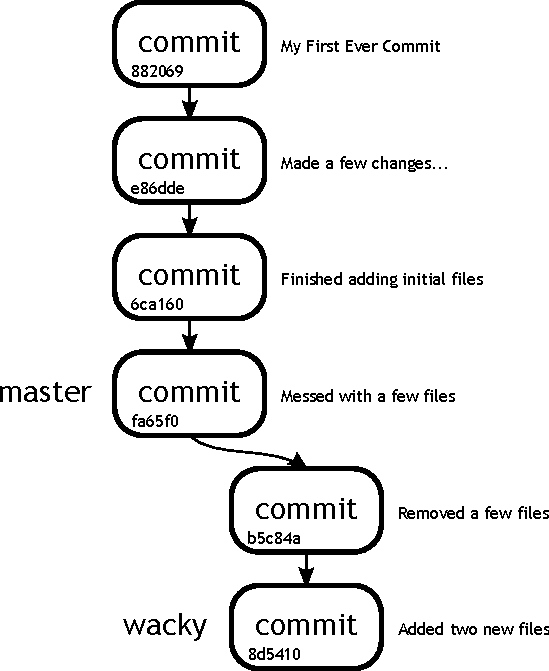
\includegraphics[width=9cm]{images/f-w4-d1.pdf}
\caption{Our first branch}
\end{figure}

So there are really two pointers in our repository at the moment, from a branch point of view.  One of them points to commit \textbf{fa65f0\ldots} and is called \textbf master.  The other is called \textbf{wacky} and points to \textbf{8d5410
\ldots}.  At this point you may be thinking that branches are pretty much the same thing as tags.  Well, they are except for one important fact.  We are going to use our \texttt{git branch} command, with a new parameter, to show us the difference.  Take a look at the output of the following operations.  We have pruned the output of the \texttt{git show} command for brievity.

\begin{Verbatim}[frame=leftline,framerule=1mm,fontsize=\relsize{-3}] 
john@akira:~/coderepo$ git branch -v
  master fa65f06 Messed with a few files
* wacky  8d5140a Added two new files
john@akira:~/coderepo$ git tag v2.0
john@akira:~/coderepo$ git show v2.0
commit 8d5140aa7d2bfc43b225afd2549d180dcb16bef6
...
...
...
\end{Verbatim}

So here we have added a tag in our current branch, \textbf{wacky}, and we can see that the commit ID for the tag \textbf{v2.0} points \textbf{8d5140a}.  We can also see that the branch \textbf{wacky} is currently pointing to the same commit ID, \textbf{8d5140a}.  Now let us add another file in, make a commit and see what happens after this.

\begin{Verbatim}[frame=leftline,framerule=1mm,fontsize=\relsize{-3}] 
john@akira:~/coderepo$ echo "New stuff" > another_file
john@akira:~/coderepo$ git add another_file
john@akira:~/coderepo$ git commit -m 'Added another file'
[wacky f91f31e] Added another file
 1 files changed, 1 insertions(+), 0 deletions(-)
 create mode 100644 another_file
john@akira:~/coderepo$ git show v2.0 
commit 8d5140aa7d2bfc43b225afd2549d180dcb16bef6
...
...
...
john@akira:~/coderepo$ git branch -v
  master fa65f06 Messed with a few files
* wacky  f91f31e Added another file
john@akira:~/coderepo$ 
\end{Verbatim}

How interesting.  The difference between tags and branches now becomes pretty clear.  Whilst a tag always points to the same commit, a branch reference always points to the tip of that branch.  In essence the reference that a branch points to moves as subsequent commits are made.  By doing this, the whole history of the branch can be retraced.  Since we know the latest commit, we also know the parent of that commit and so on and so on.

Since a branch is just a pointer to a commit, performing operations like adding, modifying and deleting files in the repository can be done safely, without destroying any data in another branch.  In short, it will allow us to completely redesign whatever is being stored in the current branch without worrying about how it will affect our baseline.  For a developer, this is pretty crucial stuff.  This gives people the chance to play with their data and experiment, which is often where the greatest ideas come from.

\section{Day 2 - ``Branches galore''}
\subsection{Working with branches}

Now we know about branches in general, we should really learn about how to merge changes from one branch into another.  Branches are fantastic for trying new things out and testing ideas, but if those ideas are successful, we need a way of pulling those changes into our \textbf{master} branch.  

Of course we could do this the old fashioned way.  We could switch into our \textbf{wacky} branch, do a little development, copy the files somewhere else, switch to our \textbf{master} branch, and paste the files over the top.  Now, this is probably the simplest way of merging possible.  In actual fact, this is not really merging at all.  However one thing that would be lost is the history of how that branch has developed over time.  Sometimes this can be crucial for knowing why certain things were changed during the development process.

Let us take a litle look at the command output of a simple merge, explain it a little, and then look at a diagramatic representation.

\begin{Verbatim}[frame=leftline,framerule=1mm,fontsize=\relsize{-3}] 
john@akira:~/coderepo$ git branch
  master
* wacky
john@akira:~/coderepo$ 
\end{Verbatim}

Firstly we check just to see what branch we are on.  Next we checkout the branch we want our development branch to be merged into.  In this case, we want to merge \textbf{wacky} into \textbf{master} and so we must first checkout the \textbf{master} branch.  Then we can merge in the changes from our \textbf{wacky} branch.

\begin{Verbatim}[frame=leftline,framerule=1mm,fontsize=\relsize{-3}] 
john@akira:~/coderepo$ git checkout master
Switched to branch 'master'
john@akira:~/coderepo$ 
\end{Verbatim}

Now we can run the actual merge.

\begin{Verbatim}[frame=leftline,framerule=1mm,fontsize=\relsize{-3}] 
john@akira:~/coderepo$ git merge wacky 
Updating fa65f06..f91f31e
Fast-forward
 another_file             |    1 +
 my_first_committed_file  |    1 -
 my_second_committed_file |    1 -
 newfile1                 |    1 +
 newfile2                 |    1 +
 5 files changed, 3 insertions(+), 2 deletions(-)
 create mode 100644 another_file
 delete mode 100644 my_first_committed_file
 delete mode 100644 my_second_committed_file
 create mode 100644 newfile1
 create mode 100644 newfile2
john@akira:~/coderepo$
\end{Verbatim} 

We can see that the first line after our command shows us which commit \textbf{master} is the latest common ancestor to both branches and then which commit is the last in our new branch.  In this case we are merging from \textbf{fa65f06} to \textbf{f91f31e}.  The line below this is even more important.  This type of merge is called a \emph{fast-forward} merge.  We have not made any changes to our \textbf{master} branch since we began developing and subsequently, after finishing our development work, we literally only require fast-forwarding the \textbf{master} branch to the same point in time as our \textbf{wacky} one.  Beneath this text, we see more information about just what is included in the merge.  

We are going to perform a quick check, to see that we are in fact on the master branch and that the latest log message is the one from the point we last left the \textbf{wacky} branch.

\begin{Verbatim}[frame=leftline,framerule=1mm,fontsize=\relsize{-3}] 
john@akira:~/coderepo$ git log -n1
commit f91f31ee594ff9edade7675dd0991b9c0f7c469b
Author: John Haskins <john.haskins@tamagoyakiinc.koala>
Date:   Wed Mar 16 19:21:46 2011 +0000

    Added another file
john@akira:~/coderepo$ git branch
* master
  wacky
john@akira:~/coderepo$ 
\end{Verbatim}

Now let us take a quick look at a diagram to see how this change actually affected the commit flow.  We have included tags in this diagram, so that you can see where they point to as well.

\begin{figure}[hbt]
\centering
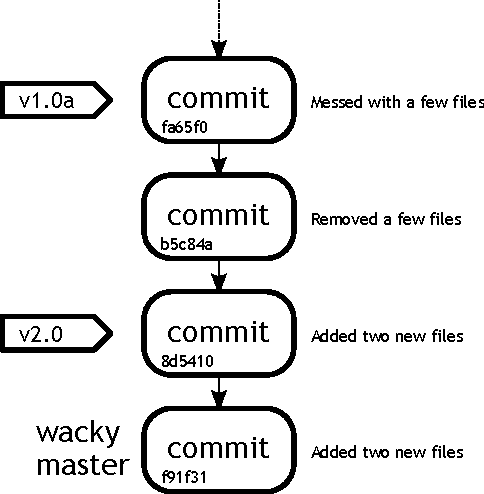
\includegraphics[width=9cm]{images/f-w4-d2.pdf}
\caption{Our first merge}
\end{figure}

This picture should make it clear that the fundamental difference between tags and branches is that whilst the pointer to a branch moves with each commit to that branch, a tag points to a single commit only and never changes, unless forcibly so by the user.

\section{Day 3 - ``Tricking the twigs''}
\subsection{Neat ways to work with branches}

There are a number of tricks that we can employ when using branches.  They are possible because of the super flexible way in which branches are implemented in Git.  As a branch is literally a pointer to a commit, certain operations are available to a user that other systems just can not implement.  However, we should point something out at this point.  Even though we have not yet made any of our repositories public or available to other people, something should always be in the back of your mind.  Allow a few minutes to read the paragraph below.

As someone once said, ``With great power, comes great responsibility.''  Git is hugely powerful.  However, with this power comes a certain level of responsibility.  We are referring here to Git's ability to change history.  If you have watched any science fiction films involving time travel, you should be aware of the difficulties and problems often associated with time travel.  In Git, the same rule applies and the basics of the rule boil down to this: \textbf{If you have made a commit, or path of commits available, you should never ever change anything in the history of those commits or the commits themselves.}  

If you are wondering why this is so important, consider this.  If you are making a series of films, and you have already released the first two of a trilogy, you would not put elements in the third one that contradict the history of the others.  You can not just act like the history of the first two did not happen.  Occasionally this happens in the film industry and what is the reaction of the public?  People get mad.  Sometimes very mad.  This is what will happen if you do the same with Git.  People who are using your repository will end up with many problems and inconsistencies.  \textbf{Do NOT do it, ever}.  There are ways to revert certain behaviour and we will cover this at a later stage.

Having said this, you should not shy away from the awesome capabilities of Git.  We are going to cover a few situations now which you may find yourself in.  Some of them do alter history, some of them do not.  This is why it is important to have an understanding of how Git works.  It can be your best friend, but it can also cause you issues.  If you take the time to tame the beast, it will be one of the most awesome tools in your developers tool bag and can save your life time and time again.  

\begin{trenches}
``Oh man.'' The familiar cry of Simon needing something reverberated round the office.  Rob could never understand why he didn't ask for help.  Simon would sit there wallowing out loud until someone could take it no longer and would eventually go over and help him.

``What to do\ldots what to do.''

Rob could take it no more.  Simon had been exclaiming now for about five minutes and Rob seemed to either be the only one who wasn't listening to music, or who was getting annoyed.  He rolled his eyes, ``What's up Si?''

Simon grinned inanely to himself.  ``I just started modifying some files and well \ldots I don't want to get rid of them \ldots I'm not 100\% sure what I've changed.  I wish I had started this in a new branch.''

``Well, when did you last commit?''

``Just before I started all this work,'' came the reply.

Rob pointed at Simon's screen.  ``You can just create a new branch now and move all the changes into it in one go.  You can do it in one command actually.''
\end{trenches}

It is one hundred percent true.  How many times have you been working on something and wished that you could move all the changes you had made to a new safe environment to protect your already good, working code.  Well, the new safe environment we spoke of sounds suspiciously like a branch.  In Git, any changes you have in your working copy can be taken into a new branch by issuing one command.  It is important to note that these changes can also be taken into an existing branch, but you may run into problems if those changes conflict with items already in that branch.

For now let us see how we can take our working copy changes into a new branch to continue development of some wonderful new feature.  We are going to start by making some changes to our newfiles.

\begin{Verbatim}[frame=leftline,framerule=1mm,fontsize=\relsize{-3}] 
pete@satsuki:~/coderepo$ echo "and some more changes" >> newfile1
pete@satsuki:~/coderepo$ echo "and a new feature" >> newfile2
\end{trenches}

Now we are going to make a new branch and switch into it.

\begin{Verbatim}[frame=leftline,framerule=1mm,fontsize=\relsize{-3}] 
pete@satsuki:~/coderepo$ git checkout -b wonderful
M	newfile1
M	newfile2
Switched to a new branch 'wonderful'
pete@satsuki:~/coderepo$ 
\end{Verbatim}

Did you see that?  We managed to create a new branch and move into it in one go.  The \texttt{git checkout} command is usually what we would use to move into a branch, not create it.  When we use the \texttt{-b} parameter, the \texttt{git checkout} command can be used to create a new branch and switch to it in one go.  Notice we have chosen the name \textbf{wonderful} for this particular branch.  There is also a status output below this that shows we have pulled two modifications into this branch, denoted by the letter \texttt{M} in front of the file name.

Now we can commit these changes.

\begin{Verbatim}[frame=leftline,framerule=1mm,fontsize=\relsize{-3}] 
pete@satsuki:~/coderepo$ git commit -a -m 'Fantastic new feature'
[wonderful f0cbf32] Fantastic new feature
 2 files changed, 2 insertions(+), 0 deletions(-)
pete@satsuki:~/coderepo$ git diff master wonderful
diff --git a/newfile1 b/newfile1
index 24e7dfa..ef20984 100644
--- a/newfile1
+++ b/newfile1
@@ -1 +1,2 @@
 A new file
+and some more changes
diff --git a/newfile2 b/newfile2
index cba16cc..dac4357 100644
--- a/newfile2
+++ b/newfile2
@@ -1 +1,2 @@
 Another new file
+and a new feature
pete@satsuki:~/coderepo$ 
\end{Verbatim}

After running the diff, we can see the differences between the \textbf{master} and the \textbf{wonderful} branches.  Looking more closely at the hunks, the only differences between the two branches are those that we made before we created our \textbf{wonderful} branch.  



MAKE CHANGES IN MASTER THEN CONFLICT

MAKE A NEW COMMIT AND MOVE IT TO A NEW BRANCH

DELETE THE BRANCH RECOVER IT

BRINGING CHANGES TO new BRANCH

DO THE WHOLE AHHH I HAVE STUFF I WANT IN A NEW BRANCH
THEN DO THE SAME WITH A COMMIT
THEN STASH


\section{Day 4 - ``Conflicting information''}
\subsection{What to do when it all goes wrong}

The team have been playing with branches for a few days now and are beginning to settle into the idea of branching often.  As you can see, in Git, a branch is a really simple device for allowing experimentation.  As the implementation of branches is so simple, it is also really fast to switch between branches.  If you have been keeping up with the After Hours sections, you can hopefully see that when switching branches, Git only needs to alter what is different between one working copy and another.


branch
checout
log -n1
branch -v
show
merge
checkout -b

\clearpage

\section{Summary - John's Notes}
\subsection{Commands}
\begin{itemize}
\item\texttt{git branch <branch_name>} - Creates a new branch with a given name

\item\texttt{git checkout <branch_name>} - Switches to a new branch

\item\texttt{git log -n1} - Limits the output of the log command to only a single line

\item\texttt{git branch -v} - Verbosely list all local branchs

\item\texttt{git show <reference>} - Show the information pointed to by the reference

\item\texttt{git merge <branch_name>} - Merge in a given branch to the current one

\item\texttt{git checkout -b <branch_name>} - Create a new branch and switch into it in one go

\end{itemize}

\subsection{Terminology}
\begin{itemize}
\item Need to think of some !!!!!!!!!!!!!
\end{itemize}
